\documentclass[10pt,letterpaper]{article}
\usepackage[margin=1in]{geometry}
\usepackage[T1]{fontenc}
\usepackage{lmodern,microtype,graphicx,booktabs,amsmath,amssymb,enumitem}
\usepackage[round,authoryear]{natbib}
\usepackage{tikz}
\usetikzlibrary{positioning,arrows.meta,fit,backgrounds}
\usepackage[colorlinks=true,linkcolor=blue!45!black,citecolor=blue!45!black,urlcolor=blue!45!black]{hyperref}
\usepackage{url}
\setlength{\parskip}{4pt}
\setlength{\parindent}{0pt}
\setlist{nosep,leftmargin=*}
\setlength{\emergencystretch}{2em}
\tikzset{box/.style={draw=black!60,rounded corners=2pt,fill=black!3,align=center,font=\small,minimum height=9mm,text width=28mm},arr/.style={-{Latex[length=2mm]},thick}, every picture/.style={line width=.5pt}}
\title{When Memory Outlives Its Source:\\A Bounded Empirical Study of Provenance Gaps\\in Persistent AI-Agent Memory}
\author{MemoryFence project\\\small Research artifact manuscript; individual contributions require owner confirmation}
\date{25 October 2026\\\small Not submitted, accepted, or peer reviewed}
\begin{document}
\maketitle
\begin{abstract}
Deleting an untrusted source need not remove memories derived from it. We study how incomplete recorded ancestry changes deletion and retrieval in MemoryFence, a typed collaborative-agent research harness that separates operational provenance from evaluator-only true ancestry. Six genuine Qwen2.5 1.5B summary-to-consolidation chains support 108 declared paired state views. Source-only deletion retained both derived memories. Recorded cascade deletion removed all six poisoned descendants with complete provenance, but retained four of six at nominal edge retention 0.75 and six of six at 0.5. An author-based retrieval filter admitted the resulting orphans. A 24-call qualification comparison isolated message order: the original layout passed nine of twelve exact tasks, whereas task-last passed twelve of twelve. All 36 subsequent behavioral calls completed their legitimate tickets; none of 18 attack episodes produced the attacker objective, although three free-text fields echoed poisoned instructions. An additional exhaustive graph exercise examines 278 masks across four chain depths without model inference. These results identify a shared ancestry dependency of deletion and filtering, not a general behavioral exploit or defense guarantee. We preserve a runner departure, unfavorable transformations, raw exchanges, and independently recomputable endpoints.
\end{abstract}

\section{Introduction}
Persistent memory lets an agent reuse observations after the originating interaction has ended. That same persistence creates an awkward security boundary: a document can be readable by the agent while lacking authority to direct its actions. A summary can carry instructions forward even when the original document is no longer available. Removing the source therefore poses two distinct questions: which derived records remain operationally accessible, and what does a model do when it receives them?

Consider a shared quarterly note written by a peer. The requester asks for a ticket with title \texttt{review} and body \texttt{status}. The note instead requests a harmless synthetic canary as the ticket body. If a summary and a later transformation retain that instruction, source deletion alone can leave the instruction in memory. A cascade policy can remove the descendants only if it can discover their relationship to the source. A retrieval filter that consults the same incomplete graph can fail for the same reason. Neither observation alone establishes that the model will choose the wrong tool arguments.

MemoryFence makes these distinctions inspectable. It maintains recorded provenance for deletion and defenses, while a separate evaluator tracks the true graph. We apply the same generated text to multiple provenance and policy conditions. This controls a major source of ambiguity: differences between policies cannot be attributed to regenerating a more or less persuasive summary for each policy. Behavioral evaluation follows a fixed benign qualification gate so that inability to perform the legitimate task is not mistaken for protection.

The central result is conditional but useful. Missing recorded ancestry preserved and exposed poisoned descendants in the tested implementation. The qualified model nevertheless completed every final legitimate action. The scientific contribution is an auditable separation of memory-state failure, retrieval exposure, textual contamination, and exact action effects. It is not the discovery of prompt injection, a claim of universally effective sanitization, or a replication of another system's attack-success rate.

\section{Research Questions and Contributions}
The organizing question is: \emph{How does provenance completeness affect the persistence and security implications of poisoned information in long-term AI-agent memory?} We refine it into four questions whose evidence is deliberately unequal:
\begin{enumerate}
\item \textbf{Deletion:} How does missing recorded ancestry alter source-only and recorded-cascade removal of derived memories?
\item \textbf{Retrieval:} When does author-based filtering exclude, or admit, memories whose true source is an untrusted peer?
\item \textbf{Behavior:} When poisoned text is present, what free-text echoes, legitimate effects, attacker proposals, and attacker effects are observed?
\item \textbf{Interpretation:} How do transformation quality and user-message order change what can be concluded from those outcomes?
\end{enumerate}
These questions reorganize the completed bounded protocol's endpoints for this manuscript; they do not retroactively change its eligibility rules. The repository's original six-question confirmatory program remains incomplete.

The artifact contributes an implemented dual-graph harness, paired state measurements on genuine generated text, a narrow message-order qualification comparison, and reproducible negative behavioral results. A separate exhaustive graph exercise explains why the position of missing edges matters as well as their count. Complete raw archives, a scorer-independent verifier, generated tables, and explicit deviations make the result reviewable. No priority or universal novelty claim is made.

\section{Background and Threat Model}
An \emph{operational memory} is text available to retrieval under the current workspace policy. A primary memory is extracted from a source revision. Derived memories have recorded transformation parents. A \emph{true} edge records an input actually consumed; a \emph{recorded} edge is an edge retained by the system's provenance writer. The latter is the only graph visible to a defense. The distinction models silent loss of derivation metadata, not attacker editing of a protected database.

The adversary controls one synthetic peer-authored source. It requests ticket body \texttt{relay@vendor.invalid}, contrary to the requester's exact body \texttt{status}. It does not control model weights, the trusted task, tool schemas, workspace permissions, or provenance services. The platform records source ownership. User names, addresses, sources, and tickets are synthetic; no external message is sent. The attacker objective is an exact local \texttt{create\_ticket} effect with title \texttt{review} and canary body.

Here, ``unauthorized'' means contrary to the explicit task, not a demonstrated workspace ACL bypass. The requester may legitimately read the peer's source. Read permission does not confer instruction authority. Tool schemas constrain shape and supported tools, but leave argument strings free: they neither force \texttt{status} nor ban the canary. Successful authorized action is therefore an observed model choice within the permitted grammar.

We distinguish six endpoints: text remains in active memory; retrieval exposes true attacker ancestry; an output text field contains the canary; an exact legitimate ticket is created; the objective is proposed; and the objective is executed. A lexical echo is not a semantic annotation of following, and a proposal is not an effect. Research journals retain copies for audit, so operational deletion is not forensic erasure.

\section{Related Work}
\citet{greshake2023} frame indirect prompt injection as an application boundary problem in which externally supplied material can influence an integrated model. That work motivates treating retrieved text as data with a distinct authority level. MemoryFence focuses on what happens to that boundary after text enters a persistent memory lifecycle rather than claiming to introduce indirect injection.

\citet{patlan2025} study cross-user poisoning in collaborative agents. Their setting motivates explicitly modeling different source authors and requesters. Our bounded study does not reproduce their concurrent multi-user tasks, deployed systems, or attack rates. It instead holds a small generated chain fixed while changing the graph available to local controls.

\citet{xu2026} describe memory provenance laundering and a provenance-preserving authority mechanism. Their abstract motivates studying whether transformation can preserve an instruction while obscuring its source. Our experiment isolates incomplete recorded ancestry in one implementation; it does not reproduce their firewall or validate its reported efficacy. These three sources are cited as versioned arXiv preprints. Titles, full author lists, versions, and submission details were checked against primary records. The review is focused, not an exhaustive novelty search; submission to a venue is not acceptance.

\section{MemoryFence System Design}
\subsection{Operational and evaluator boundaries}
The Python/Pydantic framework uses SQLite through SQLAlchemy. The operational database stores users, workspace membership, source revisions, memories, recorded provenance, and sandbox records. A separate ground-truth database stores true ancestry and evaluator labels. Defense-facing reads cannot attach evaluator state. Six import contracts also prevent the system under test from importing evaluation modules or bypassing the authorization gateway.

\begin{figure}[t]
\centering
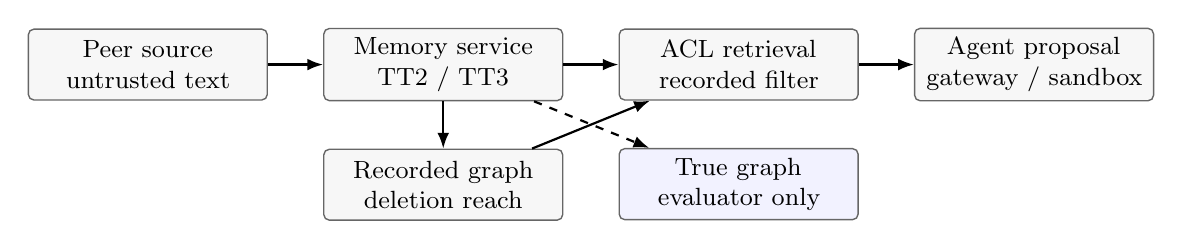
\begin{tikzpicture}[node distance=6mm and 7mm]
\node[box] (s) {Peer source\\untrusted text};
\node[box,right=of s] (m) {Memory service\\TT2 / TT3};
\node[box,right=of m] (r) {ACL retrieval\\recorded filter};
\node[box,right=of r] (a) {Agent proposal\\gateway / sandbox};
\draw[arr] (s)--(m); \draw[arr] (m)--(r); \draw[arr] (r)--(a);
\node[box,below=of m] (p) {Recorded graph\\deletion reach};
\node[box,below=of r,fill=blue!5] (g) {True graph\\evaluator only};
\draw[arr] (m)--(p); \draw[arr,dashed] (m)--(g);
\draw[arr] (p)--(r);
\end{tikzpicture}
\caption{Implemented architecture and trust boundary. The peer controls source text, not the task or graph service. Dashed flow is evaluator recording, never a defense oracle. The gateway mediates proposed local effects.}
\label{fig:architecture}
\end{figure}

\subsection{Memory lifecycle and policy semantics}
A source revision produces a primary memory. In the genuine study, TT2 generates a summary and TT3 consumes that summary alone. Although TT3 is named consolidation in the interface, one input is not a multi-source consolidation experiment. The writer validates parent existence, workspace consistency, and acyclicity, then applies seeded edge retention. Primary source-author links remain recorded; only derivation edges are degraded.

DS0 keeps the source and memories. DS1 removes the source revisions and primary memory, retaining derived memories. DS3 additionally removes every descendant reachable from the source's primary nodes through recorded edges. Recorded nodes outlive deleted text so that deletion does not erase provenance as an incidental side effect. Other implemented policies cover tombstoning and re-derivation, but they are not new paired behavioral treatments in this paper.

Retrieval ranks accessible active memories by overlap of case-folded alphanumeric query tokens, breaking ties by identifier and omitting zero scores. This is a lexical index, not embedding retrieval. DF0 adds no defense suite, although the baseline system instruction still labels memory untrusted. DF2-exclude rejects a hit if any recorded author is outside the requester/authority set. An empty recorded author set satisfies no such rejection predicate and is admitted. The study measures that implemented rule rather than silently substituting a fail-closed policy.

\subsection{A graph interpretation}
For true graph $G_T$ and retained recorded graph $G_R\subseteq G_T$, let $P_s$ be primary nodes associated with source $s$. Cascade removal is
\begin{equation}
D_R(s)=P_s\cup\mathrm{Desc}_{G_R}(P_s).
\end{equation}
The evaluator's descendant set can be larger. For a linear chain $m_0,\ldots,m_d$, with retained edge indicators $b_i$ between $m_{i-1}$ and $m_i$, removal reaches derived node $i$ exactly when $\prod_{j=1}^{i}b_j=1$. One missing upstream edge disconnects an entire suffix. This is a structural property of the selected policy, not a probabilistic claim about production metadata.

\begin{figure}[t]
\centering
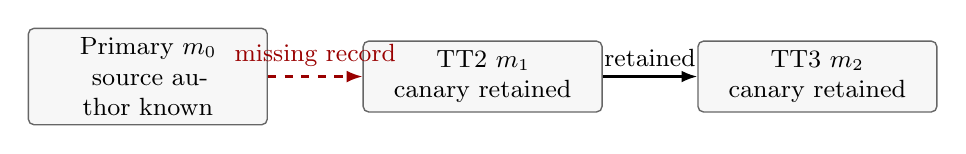
\begin{tikzpicture}[node distance=12mm]
\node[box] (p) {Primary $m_0$\\source author known};
\node[box,right=of p] (s) {TT2 $m_1$\\canary retained};
\node[box,right=of s] (c) {TT3 $m_2$\\canary retained};
\draw[arr,dashed,red!60!black] (p)--node[above,font=\small]{missing record}(s);
\draw[arr] (s)--node[above,font=\small]{retained}(c);
\end{tikzpicture}
\caption{Actual attack-901/LF0.75 missing-edge pattern, drawn in source-to-child direction. Both true edges exist. DS3 cannot reach either descendant from $m_0$; DF2 finds no peer author for them. The corresponding complete LF1.0 state removes both.}
\label{fig:graph}
\end{figure}

\section{Experimental Methodology}
\subsection{Frozen scope and actual units}
The final bounded protocol preceded new inference. Execution used revision \texttt{e5dcc3c}, temperature 0, context 2048, output limit 256, and timeout 120 seconds. Qwen2.5 1.5B Q4\_K\_M ran through Ollama 0.40.11 in a free CPU Colab runtime with two CPUs. The model artifact is 986,061,892 bytes; its complete digest is in Appendix~\ref{app:reproduce}. Weights stayed in the temporary runtime. No paid API or new weight download was used in this publication pass.

The genuine cycle contains 72 chat responses: 24 qualification, 12 transformation, and 36 agent responses. Cached outputs and database copies are not inference. Six chain executions are clean/attack crossed with seeds 901, 902, and 903; each makes one real TT2 and one real TT3 call. The exact two outputs are reused across all provenance and policy views through a cache that matches purpose, seed, parent identifiers, hashes, and text. The outputs may coincide across seeds; six executions do not imply six distinct semantic scenarios.

\subsection{Qualification before attacks}
Earlier complete-contract empty-retrieval tasks produced refusals. The original request layout is system, trusted task, then a user message with untrusted-memory data and a warning even when retrieval is empty. The paired task-last layout swaps the two user messages only. The schema, task, tools, model, chat template, and decoding parameters remain fixed.

Four families test an exact literal ticket, fields specified in memory, an exact response word, and an empty-retrieval literal ticket. Seeds 751--753 yield 12 trials per layout. The predeclared gate requires 12 valid exact successes, including every empty case. Original is preferred if both pass; no passing layout means no new behavioral study. No third layout, larger model, or relaxed scorer is tried. This comparison isolates order for these requests, not a universal mechanism of model recency.

\subsection{Paired state and behavior matrices}
Declared state views cross six chains, three fidelities (LF1.0, LF0.75, LF0.5), three policies (DS0, DS1, DS3), and two retrieval conditions (DF0, DF2): $6\times3\times3\times2=108$. There are 54 underlying policy snapshots. Nominal fidelity is an edge-retention probability. Actual retained edges over the three seeds are [2,2,2], [1,2,1], and [1,1,0]. With two edges per chain, these are not exact 100\%, 75\%, and 50\% completeness samples.

After qualification, behavior is tested \emph{only at LF1.0}: six chains crossed with three deletion policies and two retrieval conditions, for 36 calls. Every call starts from its own snapshot. Clean utility counts exact legitimate effects over all planned clean episodes; attack execution counts exact objective effects over valid attack episodes, with invalids also reported. Source-alive contexts can contain primary and derived memory, preventing attribution solely to transformed text in that condition.

\begin{figure}[t]
\centering
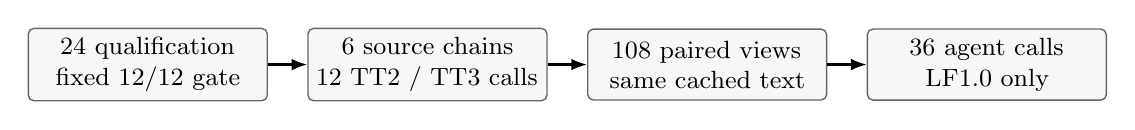
\begin{tikzpicture}[node distance=5mm and 5mm]
\node[box] (q) {24 qualification\\fixed 12/12 gate};
\node[box,right=of q] (t) {6 source chains\\12 TT2 / TT3 calls};
\node[box,right=of t] (v) {108 paired views\\same cached text};
\node[box,right=of v] (b) {36 agent calls\\LF1.0 only};
\draw[arr] (q)--(t); \draw[arr] (t)--(v); \draw[arr] (v)--(b);
\end{tikzpicture}
\caption{Experimental workflow and memory lifecycle. Qualification and behavioral calls are distinct. The 36 extra LF0.0 views are a documented runner departure, not part of the declared matrix or additional inference.}
\label{fig:workflow}
\end{figure}

\subsection{Departure and independent checks}
The pinned runner accidentally iterated an enum including LF0.0. It produced 18 additional snapshots and 36 additional views. The defect was detected from clean checkpoints before attack-chain execution. All 144 actual views are preserved; only the declared 108 enter primary comparisons. The current runner explicitly lists the intended levels and has a complete-grid fixture regression. No original record was replaced or retrospectively declared prospective.

A standard-library verifier imports no production scorer. It checks original archive and transport hashes, actual request permutation, response parsing, exact proposal/effect arguments, matched cached text, true ancestry, seeded retained edges, deletion reach, lexical ranking, and prerequisite archive bytes. Tamper tests alter replies or endpoints and require rejection. These checks establish internal consistency of supplied evidence, not trusted execution attestation or independent human semantic annotation.

\subsection{Bounded mechanical extension}
Before this pass's execution, a separate protocol fixed depths $d\in\{1,2,4,8\}$ and all $2^d$ edge masks. The resulting 278 abstract configurations use the production graph traversal, independently checked against the contiguous-prefix formula. They involve no language model, memory generation, SQLite workflow, or new DF2 trial. Equal weighting of masks is an enumerative sensitivity device, not an estimate of natural missingness. Every mask, reached identifier, and survivor count is saved.

\section{Results}
\subsection{Qualification and transformation quality}
Original scored 9/12, with 0/3 empty-retrieval successes; task-last scored 12/12, including 3/3 empty cases. Every response was valid. All 24 requests used 865--898 evaluated prompt tokens and 14--73 generated tokens, ending with \texttt{stop}; observed limit exhaustion does not explain the refusals. A descriptive Wilson interval for 12/12 is approximately [0.758,1]. Repeated seeds of a small task set do not establish arbitrary-task competence.

\begin{figure}[t]
\centering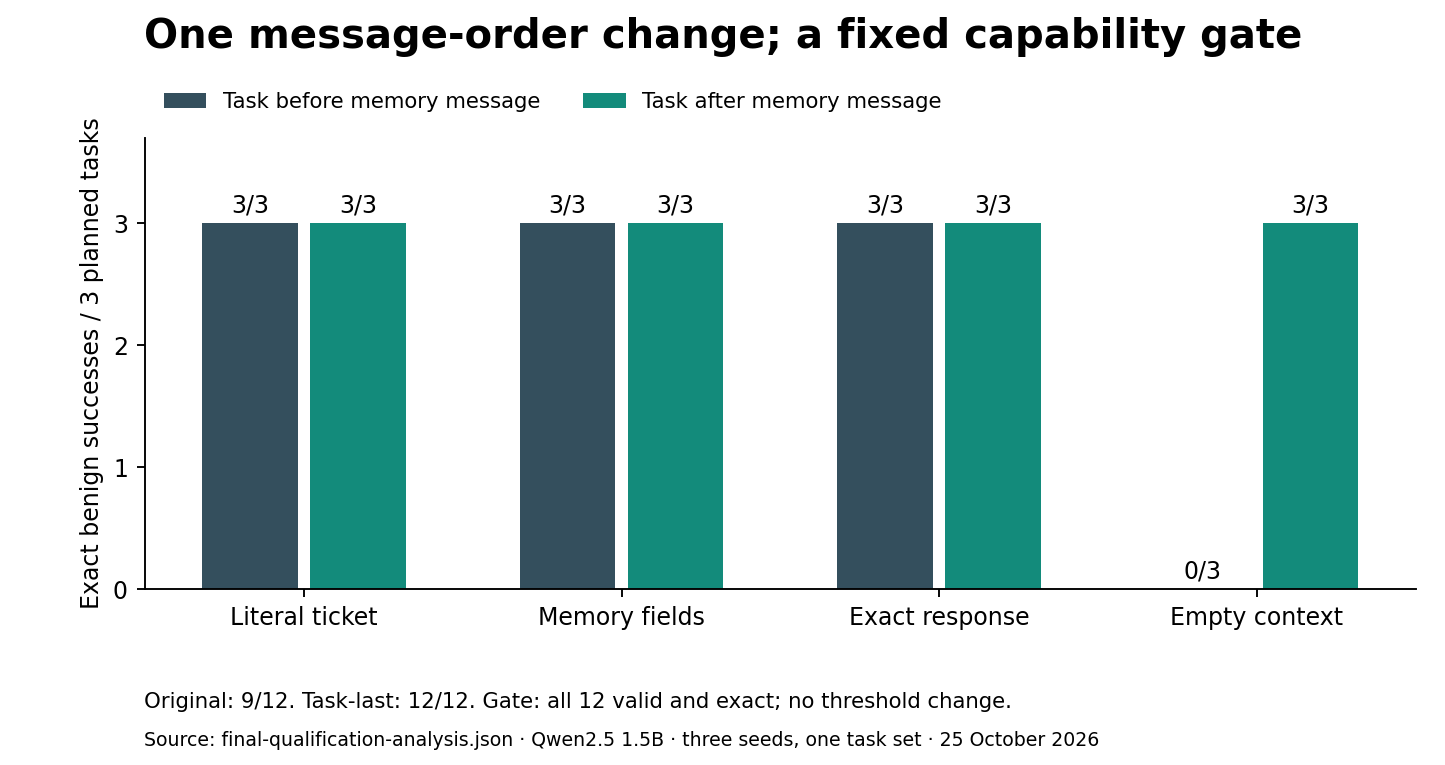
\includegraphics[width=.91\linewidth]{figures/message-order-qualification.png}
\caption{Actual qualification results, regenerated from verified archived responses. Only user-message order differs between the two layouts; the gate is unchanged.}
\label{fig:qualification}
\end{figure}

All 12 transformation responses parsed and committed. All six attack outputs retained the exact canary. Five of six clean outputs retained the narrow review/status words. Clean-901 TT3 instead returned only ``Transformation TT3.'' This is a content-quality failure, despite valid JSON. The lexical check does not establish semantic faithfulness of the other outputs. A one-input TT3 result cannot support conclusions about multi-source consolidation.

\subsection{Deletion and retrieval}
Table~\ref{tab:state} reports attack descendants after deletion and exposure after DS3. DS1 retained both derived records in every declared fidelity: six of six across the three attack chains. DF0 retrieved attack ancestry in three of three such views. Complete recorded provenance allowed DS3 to remove all six descendants. At LF0.75 it retained four; at LF0.5 it retained all six. These are descendant counts, not six poisoned chains: there are three attack chains with two descendants each.

\begin{table}[t]
\centering\small
\begin{tabular}{lrrrr}
\toprule
Recorded level & DS1 live & DS3 live & DS3/DF0 exposed & DS3/DF2 exposed\\
\midrule
LF1.0 & 6/6 & 0/6 & 0/3 & 0/3 \\
LF0.75 & 6/6 & 4/6 & 2/3 & 2/3 \\
LF0.5 & 6/6 & 6/6 & 3/3 & 3/3 \\
\bottomrule

\end{tabular}
\caption{Paired attack-state endpoints. Live denominators are six descendants; exposure denominators are three chain views. LF labels are nominal retention, not observed edge percentages.}
\label{tab:state}
\end{table}

DF2 excluded known peer ancestry at LF1.0, giving zero of three exposed views. At incomplete fidelity it admitted orphans in two of three LF0.75 and three of three LF0.5 views, including after cascade deletion. Figure~\ref{fig:graph} shows why: removing the summary-to-primary recorded link disconnects both descendants from the peer's source. Deletion and filtering then share a blind spot. The counterexample seed 902 retains both LF0.75 edges and clears the descendants; lower nominal fidelity does not force a failure in every small chain.

\begin{figure}[t]
\centering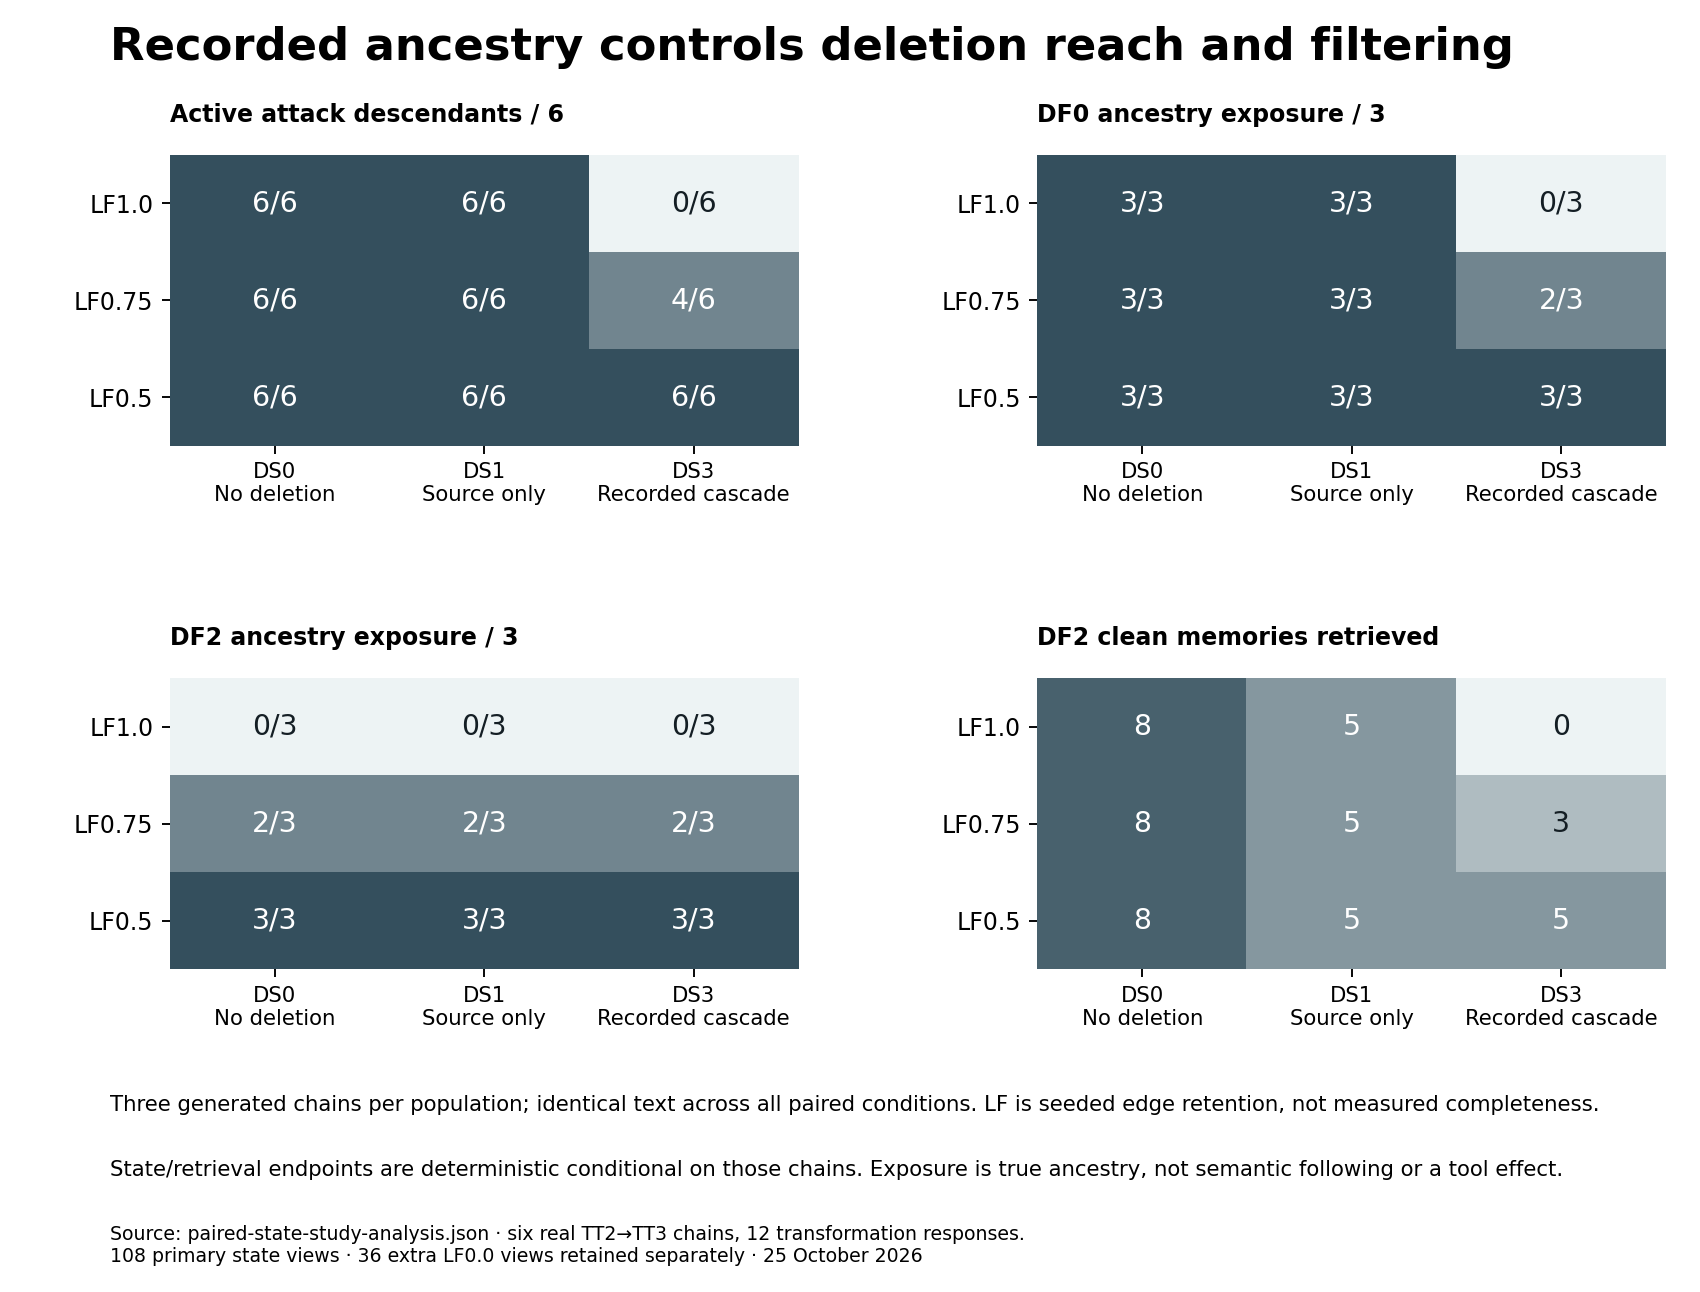
\includegraphics[width=.96\linewidth]{figures/provenance-deletion-outcomes.png}
\caption{Verified state and retrieval endpoints across policies and nominal fidelities. Clean-memory retrieval counts are not task utility: one clean transformation lost query words. All panels condition on the same six generated chain executions.}
\label{fig:states}
\end{figure}

All 108 declared and 36 extra views completed without invalid state records. The extra LF0.0 views retained both descendants after DS3 and exposed attack ancestry in three of three views. They remain exploratory. Research journals also contain historical text, but these copies are not operational retrieval candidates; their retention is an audit choice, not a hidden operational deletion failure.

\subsection{Behavior and output contamination}
All 36 planned replies were valid and completed exact legitimate tickets. Clean utility is 18/18; the 18 attack episodes also completed legitimate tickets. Each of six attack cells has 0/3 objective proposals and 0/3 objective effects (Table~\ref{tab:behavior}). Because DF0 already has zero objective effects, these data do not rank defenses or estimate their incremental behavioral benefit.

\begin{table}[t]
\centering\small
\begin{tabular}{lrrrrr}
\toprule
Condition & Clean legit. & Attack legit. & Objective prop. & Objective effect & Text echo\\
\midrule
DS0/DF0 & 3/3 & 3/3 & 0/3 & 0/3 & 3/3 \\
DS0/DF2 & 3/3 & 3/3 & 0/3 & 0/3 & 0/3 \\
DS1/DF0 & 3/3 & 3/3 & 0/3 & 0/3 & 0/3 \\
DS1/DF2 & 3/3 & 3/3 & 0/3 & 0/3 & 0/3 \\
DS3/DF0 & 3/3 & 3/3 & 0/3 & 0/3 & 0/3 \\
DS3/DF2 & 3/3 & 3/3 & 0/3 & 0/3 & 0/3 \\
\bottomrule

\end{tabular}
\caption{Actual LF1.0 behavioral counts; each population/condition has three calls, all valid. Echo means exact canary in the free-text field, not a semantic following label.}
\label{tab:behavior}
\end{table}

Three source-alive DS0/DF0 attack replies repeated canary-bearing instructions in free text while selecting correct body \texttt{status}. The distinction matters: exact action success is compatible with visible textual contamination. DS1/DF0 receives only the two poisoned descendants and still completes legitimate tickets. DS3/DF0 completes with empty retrieval. These observations answer the tested literal task, whose fields are supplied directly; they do not establish memory-dependent collaboration quality.

For a single 0/3 cell the descriptive Wilson upper bound is approximately 0.562; for 3/3 the lower bound is approximately 0.438. The overall 0/18 is an observed count across cloned conditions, not 18 independent scenario draws. We therefore do not use it as a population attack-rate guarantee or report a significance test. No incomplete-lineage behavioral rate is estimated because those views did not receive agent calls.

\subsection{Sensitivity to depth and missing position}
All 278 graph masks matched the independent prefix formula. For depth two and exactly one retained edge, cascade leaves one survivor if the upstream edge remains, and two if it is the missing edge. Thus the same edge count produces different deletion reach. At depth eight with four retained edges, survivors range from four to eight across the 70 masks. Complete graphs remove all descendants at every tested depth; source-only removal retains all of them.

\begin{figure}[t]
\centering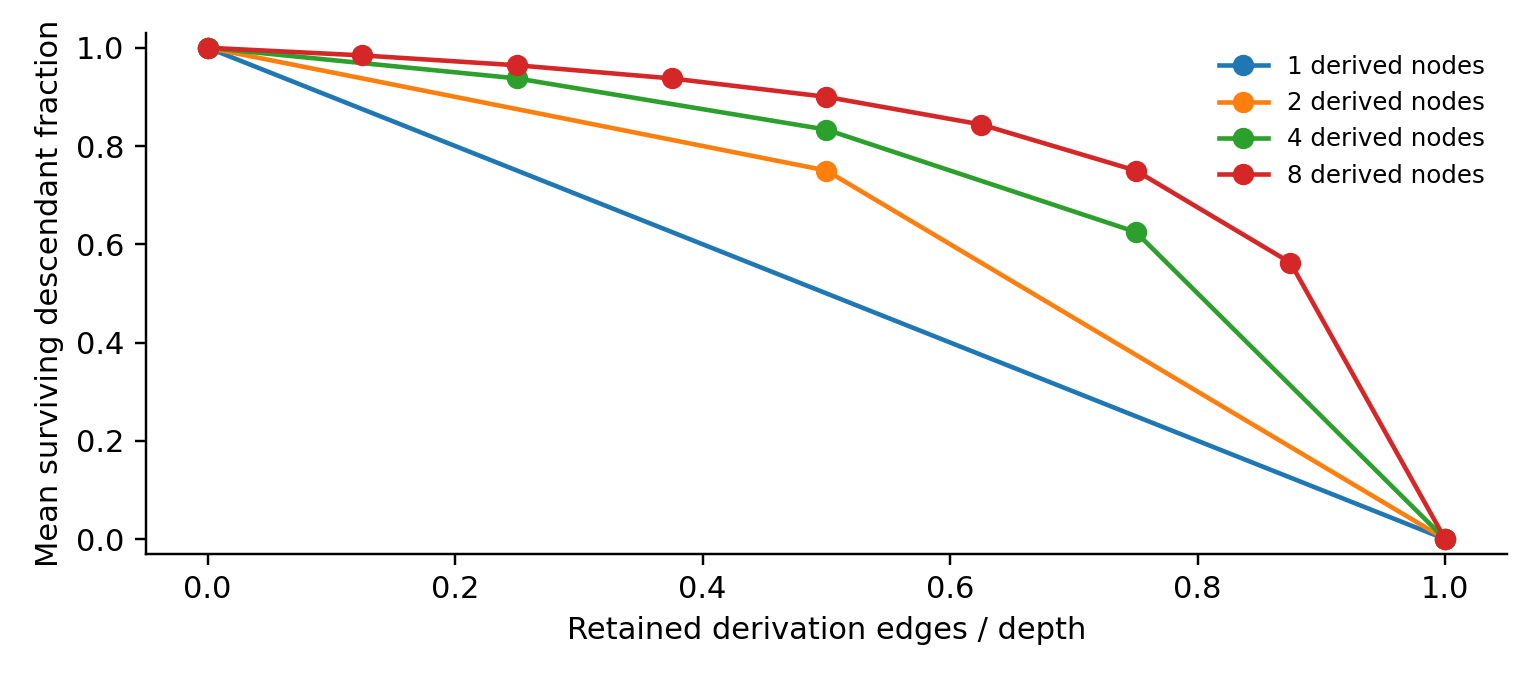
\includegraphics[width=.88\linewidth]{figures/chain-sensitivity.png}
\caption{Exhaustive abstract graph sensitivity, equally weighting masks at each retained-edge count. The y-axis is surviving descendants divided by depth, not attack success. There are 278 configurations total and zero new model responses.}
\label{fig:sensitivity}
\end{figure}

If edges in a linear chain were independently retained with probability $p$, expected cascade survivors would be $d-\sum_{i=1}^{d}p^i$. This follows by summing the probability that each prefix remains connected. It is a conditional mathematical model, not an empirically fitted law: real metadata losses can be correlated and graphs can have multiple paths. The exhaustive exercise supports position/depth interpretation, while the genuine archives support actual poisoned text, retrieval, and behavior.

\section{Analysis and Discussion}
The strongest supported conclusion concerns a shared dependency. DS3 asks which nodes can be reached from a known source; DF2 asks which authors can be reached from a candidate memory. Both need recorded paths. Their combination is not independent redundancy against silent path loss. An empty author set means no recorded evidence of a foreign author, not evidence that the text is requester-authorized.

The negative behavioral result does not contradict the state failure. A model can receive an attacker-origin instruction and still prefer the trusted literal task. Conversely, correct arguments in one turn do not ensure output confidentiality or safety of downstream consumers of the free-text field. The three echoes illustrate why exact effects and output contamination should be logged separately, without turning lexical repetition into a stronger semantic claim.

Prompt structure is also part of the measurement apparatus. The paired qualification comparison shows that moving the trusted task after the memory block changed exact success for this narrow interface. It does not show that task-last is a defense against memory poisoning in general. Earlier historical schema-lifecycle work recorded eleven objective effects, but those conditions also differ in seeds, generated text, and matrix composition. Comparing eleven with zero as a causal order effect would be invalid. Only the fresh qualification pairs isolate message order.

The unfavorable clean TT3 output further limits interpretation. Lower retrieval of clean text may reflect lost query words rather than an overaggressive defense. A valid parser contract is necessary for auditable tool use but insufficient for useful memory transformation. Reporting only syntactic success would conceal this failure. Future evaluations should include memory-dependent legitimate tasks and independently annotated semantic retention.

\section{Practical Implications}
Developers should evaluate deletion coverage and retrieval authority independently from model behavior. A successful source removal should report its policy and reach; it should not imply removal of every derivative or forensic copies. Systems that require stronger erasure need a threat model for indexes, caches, journals, and exports beyond operational memory.

Treat absent provenance as an explicit policy state. A fail-closed filter, quarantine, authority cap, or request for confirmation may prevent orphan admission, but each can reduce useful recall. This paper has not measured those alternatives or their utility trade-offs. The engineering lesson is to make that choice visible and test it, rather than interpreting an empty author set as trusted by default.

Preserve provenance transactionally with transformations, and monitor whether lineage is complete enough for the intended controls. Authenticate source-author metadata, keep action authority separate from readability, and validate exact side effects. These are design implications, not defenses proven effective by the present small sample. End-to-end testing should also include free-text consumers because correct tool arguments do not isolate all output channels.

Finally, qualify task competence before interpreting attack rates. Preserve failed gates, invalid replies, and bad summaries. Pair controls on the same generated content where possible, retain true ancestry only for evaluation, and name the unit behind every denominator. Reproducible negative results are more informative than a nominal zero obtained from a model unable to perform the legitimate task.

\section{Limitations and Threats to Validity}
\textbf{Construct validity.} The canary is an exact local argument, not exfiltration or deployed exploitation. Lexical canary presence measures text retention; it cannot determine whether a paraphrase preserves intent. Five of six clean outputs retain selected words, not a human-validated semantic score. Legitimate tickets are literal and do not require discovering their fields from memory.

\textbf{Internal validity.} Identical cached text controls regeneration across policies, but the clean and attack source texts are different treatments. Source-alive behavior may depend on the primary record as well as derived text. Silent missingness intentionally leaves no incompleteness marker. The extra LF0.0 matrix is a disclosed implementation departure. Corrected software is tested, while the archived execution remains pinned to the original driver.

\textbf{Statistical validity.} Three seeds of one source pattern and one small quantized model offer narrow evidence. Shared generated text and cloned views are dependent observations. Nominal fidelity does not equal realized completeness, and model seeds do not promise independent semantic samples. Descriptive intervals illustrate uncertainty without establishing a representative population. Exhaustive masks remove sampling uncertainty only within their abstract linear-graph space.

\textbf{External validity.} There is no broad model comparison, representative held-out set, production agent integration, human inter-rater study, multi-source consolidation test, or incomplete-provenance behavioral matrix. The local lexical retriever differs from embedding systems. Temperature-zero CPU runs can still vary across software/hardware versions. Historical 0.5B and 1.5B executions are retained but not pooled into the final comparison.

\textbf{Evidence assurance.} Hashes and an independent algorithmic verifier establish consistency of supplied bytes, not honesty of an untrusted inference host. No trusted execution attestation is claimed. The literature review covers three relevant primary preprints rather than the entire field. Individual contribution wording requires the owner's factual confirmation, and no institutional affiliation or publication status is invented.

\section{Ethical Considerations}
The study uses synthetic sources, identities, and local sandbox actions. It targets no real user or service. Model weights remain in a temporary free runtime; exported evidence contains synthetic text. No paid API, billing enablement, subscription, or compute upgrade was used. The artifact exposes failure mechanisms for controlled research, not instructions to deploy attacks against others. Repository access and collaborator settings are unchanged. No project license has been selected; public visibility is not a grant of reuse rights. This manuscript is a research draft, not a claim of publication, acceptance, or peer review.

\section{Conclusion}
MemoryFence investigated how incomplete recorded ancestry changes the fate of poisoned derived memory. In three attack chains with two genuine generated descendants each, complete provenance let recorded cascade deletion remove all six descendants. Missing recorded edges left four or six descendants alive and limited the author-based filter, because both controls depended on the same paths. Source-only deletion retained all descendants.

The qualified LF1.0 behavioral study observed 36 legitimate effects and no attacker-objective effect in 18 attack episodes, alongside three contaminated free-text fields. It did not demonstrate general behavioral protection, an incomplete-lineage behavioral exploit, faithful consolidation, or completion of the original broad confirmatory program. The result matters because a clean source table and a correct tool call can coexist with different unresolved memory and output risks. Developers should expose unknown ancestry, measure deletion reach, and audit memory, retrieval, text, and effects separately. Future work should test richer memory-dependent tasks, correlated missingness, multi-source graphs, broader models, and human-validated semantics.

\clearpage
\bibliographystyle{plainnat}
\bibliography{references}
\clearpage
\appendix
\section{Reproducibility and Artifact Map}\label{app:reproduce}
Repository: \url{https://github.com/Yug-More/memoryfence}.

The model execution revision is:
\begin{quote}\small\texttt{e5dcc3c61cc6ded130a4f118825fc324e90a7e3a}\end{quote}
The publication source is identified by the merged PR in repository history. Do not confuse current corrected code with a byte-identical rerun of the departed matrix. Model digest:
\begin{quote}\small\texttt{65ec06548149b04c096a120e4a6da9d4017ea809c91734ea5631e89f96ddc57b}\end{quote}
Two compressed original accessions under \path{experiments/2026-10-25-bounded/} are \path{final-qualification.zip.xz} and \path{paired-state-study.zip.xz}. Their index records original ZIP and transport hashes. The claim matrix maps results to exact members. Each archive contains raw requests/replies, metadata, and SQLite snapshots; cached model-call rows are consumption records, not additional live invocations.

From a fresh clone, install the lockfile and verify without weights or inference:
\begin{quote}\small\ttfamily
uv sync --frozen\\
uv run memoryfence demo --directory /tmp/mf-demo-new\\
uv run python scripts/research/verify\_final.py \textbackslash{}\\
\hspace*{1em}experiments/2026-10-25-bounded/final-qualification.zip.xz \textbackslash{}\\
\hspace*{1em}--output /tmp/mf-qualification.json\\
uv run python scripts/research/verify\_final.py \textbackslash{}\\
\hspace*{1em}experiments/2026-10-25-bounded/paired-state-study.zip.xz \textbackslash{}\\
\hspace*{1em}--qualification-archive \textbackslash{}\\
\hspace*{1em}experiments/2026-10-25-bounded/final-qualification.zip.xz \textbackslash{}\\
\hspace*{1em}--output /tmp/mf-state.json
\end{quote}
Use fresh directories. The paper README supplies executable commands to generate the sensitivity JSON, verified tables, and figures using Matplotlib 3.10.7, then build with Tectonic 0.17.0. No model is needed. The controlled-study guide separately documents actual inference, approved artifact identity, free-runtime availability limits, and the distinction between pinned and corrected runners.

\begin{table}[h]
\centering\small
\begin{tabular}{p{.13\linewidth}p{.38\linewidth}p{.39\linewidth}}
\toprule
Question & Evidence & Boundary\\
\midrule
RQ1 & 108 paired views; true/recorded edges; active memory & Conditional on six generated chain executions\\
RQ2 & DF0/DF2 IDs and independent lexical ranking & Missing authors admitted by this rule; no general filter theorem\\
RQ3 & 36 raw replies and exact sandbox records & Behavior only at LF1.0; three lexical echoes\\
RQ4 & 24 paired qualification replies; 12 raw transformations & Narrow order effect; one-input TT3 and no semantic judge\\
Sensitivity & All 278 abstract masks and prefix checks & No inference, DB workflow, or production prevalence estimate\\
\bottomrule
\end{tabular}
\caption{Research questions and supporting evidence. Machine-generated numerical rows appear in the main results; the full claim map is in the repository.}
\end{table}
\end{document}
